\scanpage{268}
\uline{Corollaire} 2.3 Supposons $\dim X_0\leq1$. Alors $X$ est projectif sur $Y$.
\margin{\figure{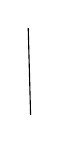
\begin{tikzpicture}\draw (0,1.1)--(.03,0);\end{tikzpicture}}}

\uline{Corollaire} 2.4. Soit $A$ comme dessus \inserted{et \uline{réduit}}, soit $Y=\operatorname{Spec}A$, $\widetilde Y=\operatorname{Spec}(\widehat A)$, $y$ ($\widetilde y$) le pt fermé de $A$. \inserted{Supposons $y$ singularité \uline{isolée}} Alors l'hom $\operatorname{Pic}(Y-y)\to\operatorname{Pic}(\widetilde Y-\widetilde y)$ est un \uline{\deleted{\unsure{mono}}\inserted{iso}morphisme}.
\figure{\begin{tikzpicture}[x=1cm,y=1cm]\draw (0,2.1)--(.03,0);\draw (6.8,2.4)..controls(6.5,1.6)and(6.8,1.4)..(7.8,1.4)--(8.4,1.45)--(8.3,1.05);\draw (6.8,2.4)--(11.2,2.4)..controls(11.5,1.8)and(11.3,1.5)..(11,1.45)--(8.4,1.45);\end{tikzpicture}}

\deleted{Cet hom est injectif}

On peut supposer que les composantes irred. de $Y$ soient de dim $\geq2$. Alors, pour tt Module loc. libre $E'$ sur $Y'=Y-\{y\}$, $i_*(E')$ est coh (i.e. $i:Y'\unsure{\text{---}|\to}Y$ l'imm. can)

\margin{\unsure{dégager un énoncé plus général} valable si $A$ est \unsure{quotient d'un|localisé d'un} \unsure{régulier|schéma}, \deleted{\unsure{excellent|noethérien}}}

En particulier, $i_*(\mathcal O_{Y'})$ est cohérent, donc correspond à une algèbre $A'$ finie sur $A$. \deleted{Rien ne change \unsure{à|si}} Cette dernière correspond à un $\unsure{Y_1|X_1}$ fini sur $\unsure{Y|X}$, réduit, tq que
\[
Y'_1=Y_1|Y'\to Y'\text{ soit un isom},
\]
[donc $\widetilde Y'_1=\deleted{\unsure{Y_1}}\inserted{\widetilde Y_1|\widetilde Y'}\to\widetilde Y'$ est \deleted{\unsure{tel que}} un isom], \deleted{et $\unsure{Y_1}\;\Gamma($} et
\[
\Gamma(Y_1)\to\Gamma(Y'_1)\text{ est un isom}.
\]
\margin{\figure{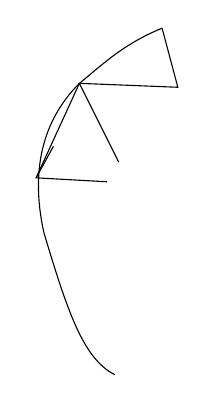
\begin{tikzpicture}[x=1cm,y=1cm]
\draw (1.5,3.8)--(1.7,3.05)--(.45,3.1)..controls(.05,2.7)and(-.2,2.1)..(0,1.2)..controls(.3,.2)and(.5,-.4)..(.9,-.6);
\draw (1.5,3.8)..controls(1,3.6)and(.7,3.3)..(.45,3.1)--(.95,2.1);\draw (.45,3.1)--(-.1,1.9)--(.8,1.85);\draw (-.1,1.9)--(.12,2.3);
\end{tikzpicture}}}
Car nous revenons au cas où $\Gamma(Y_{\unsure{1}})\to\Gamma(Y')$ est un isom, i.e. à $\operatorname{prof}A\geq2$. Un raisonnement facile

\mspage{267}
